\documentclass{book}
\usepackage{mathtools}
\usepackage{tikz}
\usetikzlibrary{positioning}

\usepackage{amsthm}
\usepackage{amsmath}
\usepackage{amssymb}

\newtheorem{defn}[equation]{Definition}
\newtheorem{coro}[equation]{Corollary}
\newtheorem{prop}[equation]{Proposition}
\newtheorem{prf}[equation]{Proof}
\renewenvironment{proof}{\emph{Proof}.}{\qed}


\begin{document}

\tableofcontents

\chapter{Mathematical representation of physical objects}



\section{Manifolds and continuous quantities}
\emph{We tell physical object apart by identifying some measurable properties. In particular, we are interested in properties that are continuous quantities. This gives us manifolds.}

\subsection{Physical objects and quantities}

- \emph{There is a physical object that we want to identify}

Say we're looking at weather. We'll want to know the temperature, wind speed, humidity, whereabouts, etc.

- \emph{We can say it lives in some subset of possibilities, and can give real number values corresponding to that subset. This gives us quantities}

Fahrenheit, mph, percent humidity, location.
On some set of all possible weather configurations, we look at a specific subset of possibilities. This is our weather report.  

Talking about location on the earth, a \textbf{single space cannot cover the entire earth such that a consistent set of quantities will be defined}. The poles must be in two separate subsets, with separate quantities. 

\begin{defn}
	A \textbf{quantity} is an function $q : U \to \mathbb{R}$ that assigns a measurable value to a physical object.
\end{defn}


- \emph{Having a set of one-to-one quantities sufficient to distinguish one object from another, but not so many that some end up redundant, gives us a coordinate system}


\begin{defn}
	A \textbf{coordinate system} $[q]$ is a collection of $n$ quantities $q^i : U \to \mathbb{R}$ such that there is a one-to-one relationship between the physical objects in $U$ and the values of the quantities in $\mathbb{R}^n$.
\end{defn}


- \emph{\textbf{Overlapping} coordinate systems can be transformed between}

TODO: add the diagram (use Tikz)

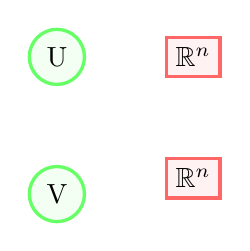
\begin{tikzpicture}
[roundnode/.style={circle, draw=green!60, fill=green!5, very thick, minimum size=7mm},
squarednode/.style={rectangle, draw=red!60, fill=red!5, very thick, minimum size=5mm},
]
\node[roundnode]	(U) {U};
\node[roundnode]	(V) [below=of U]{V};
\node[squarednode]	(realU) [right=of U] {$\mathbb{R}^n$};
\node[squarednode]	(realV) [below=of realU] {$\mathbb{R}^n$};
\end{tikzpicture}

\begin{defn}
	Given two coordinate systems  $[q] : U \to \mathbb{R}^n$ and $[p] : V \to \mathbb{R}^n$ such that $U \cap V \neq \emptyset$, we call a \textbf{coordinate transformation} the function $f = [p] \circ ([q])^{-1} : \mathbb{R}^n \to \mathbb{R}^n$.
\end{defn}




- \emph{Now that we have sets that can be mapped to the real numbers, we can define manifolds}

For the weather example, a manifold would be all possible weather conditions (including things that can't necessarily be quantified, like the color of a sunset), with a subsection whereon is defined a weather report, measuring temperature, wind speed, etc. in different places. If we're looking to parametrize the entire earth, then our manifold cannot be covered with a single subset, because the earth is roughly a sphere. We will need multiple subsets to cover all of the earth, and all possible weather conditions. 


 
\begin{defn}
	A \textbf{manifold} is a set of physical objects $X$ such that for any $x \in X$ there exists a $U \subset X$ that contains $x$ and upon which a coordinate system $[q]$ is defined.
\end{defn}

\begin{defn}
	For a given manifold X, a collection of subsets of X that completely cover X are called the \textbf{atlases} of X. 
\end{defn}



\subsection{Sub-manifolds and k-surfaces}

- \emph{Within a manifold can lie a manifold of equal or smaller dimension, with a mapping between them}

If in the original weather report we were worrying about temperature, humidity, and wind speed, we could instead hold one of the three values fixed (say, humidity), and vary the other two. The latter manifold, with humidity held constant, would be a sub-manifold of the former, where all three variables are allowed to change.  



\begin{defn}
	Consider a manifold X of dimension n, and a manifold Y of dimension k, such that $k \leq n$. Y is a \textbf{submanifold} or a m-surface of X if any point on Y is also a point on X. 
\end{defn}

- parameterization of Y can be done in terms of the coordinates of X; $q^i(p^j)$

TODO: add corollary and paragraph about "parametrization"

\begin{coro}
	Suppose we have a manifold X of dimension n, with a submanifold Y of dimension k, such that $m \leq n$. Therefore, the coordinate transformation from X to Y will be onto, while the coordinate transformation from Y to X will be one-to-one. 
\end{coro}



\emph{What are the possible submanifolds of a given manifold?}


\begin{defn}
	For some manifold X of dimension n, $S^k$ is the set of all possible \textbf{k-surfaces}, or sub-manifolds of dimension $k \leq n$. 
\end{defn}

- \emph{A manifold of dimension n can have a boundary of dimension n-1. The boundary itself will not have a boundary.}

The boundary of a weather report would be readings restricted to a specific climate. 


\begin{defn}
	Given k-surface $\sigma \in S^k$, if for some point $x \in \sigma$ you can construct a open neighborhood around x in $\mathbb{R}^n$ completely within $\sigma$, then x is an \textbf{interior point} of $\sigma$. 
\end{defn}

\begin{defn}
	Given k-surface $\sigma \in S^k$, if some point $x \in \sigma$ is not an interior point, then $x$ is a \textbf{boundary point}.
\end{defn}

\begin{defn}
	Given k-surface $\sigma \in S^k$, $\partial\sigma \in S^{k-1}$ is the set of all boundary points of $\sigma$, or, the \textbf{boundary} of $\sigma$. 
\end{defn}

- \emph{Dimension is one less since at each section of the boundary, one of the dimensions must be held fixed. }

- \emph{$\partial\partial\sigma$ is empty since all points on the boundary are interior with respect to the boundary}


\begin{coro}
	Given $\sigma \in S^k$, $\partial\sigma \in S^{k-1}$, and $\partial\partial\sigma = \emptyset$. 
\end{coro}

TODO: parametrization of the boundary (\emph{consider a cube, rather than a ball})

- The boundary appears to be very similar to a line, in that all points on the boundary are interior with respect to the boundary. 

\subsection{Linear Functionals of K-surfaces}


\begin{defn}
	A \textbf{linear function of k-surfaces}, or \textbf{k-functional}, is a function $F : S^k \to \mathbb{R}$ such that for $\sigma_1$, $\sigma_2 \in S^k$, if $\sigma_1 \cap \sigma_2 \subseteq \partial\sigma_1 \cup \partial\sigma_2$, then $F(\sigma_1\cup\sigma_2) = F(\sigma_1) + F(\sigma_2)$. 
\end{defn}


Given $F : S^k \to \mathbb{R}$, we can then define $G : S^{k+1} \to \mathbb{R}$ such that $G(\sigma) = F(\partial\sigma)$, and $H : S^{k+2} \to \mathbb{R}$ such that $H(\sigma) = G(\partial\sigma) = F(\partial\partial\sigma)$. 

\begin{prop}
	A k-functional applied to the empty set gives zero. 
\end{prop}
\begin{proof}
	Let $F : S^k \to \mathbb{R}$ be a linear function. Consider the empty set $\emptyset$. 
We have $\emptyset \cap \emptyset \subseteq \partial\emptyset \cup \partial\emptyset$, and $\emptyset = \emptyset\cup\emptyset$. 
So, $F(\emptyset) = F(\emptyset\cup\emptyset) = F(\emptyset) + F(\emptyset) \implies F(\emptyset) = 2F(\emptyset) \implies F(\emptyset) = 0$
\end{proof}


\begin{defn}
	For $F : S^k \to \mathbb{R}$ and k-surface $\sigma$, we say that $\partial F(\sigma) \equiv F(\partial\sigma)$. 
\end{defn}

\begin{coro}
	For $F : S^k \to \mathbb{R}$ and $G : S^{k+1} \to \mathbb{R}$, since $F(\partial\sigma) = \partial F(\sigma)$, $\partial F(\sigma) = G(\sigma)$. 
\end{coro}

\begin{prop}
	Let $F \in F_k$ be a k-functional, then $\partial\partial F = 0 $.
\end{prop}
\begin{prf}
	We want to show that a linear functional applied to a surface whereon the boundary operator was applied twice will always give zero.
	
	Let $F : S^k \to \mathbb{R}, G : S^{k+1} \to \mathbb{R}, and H : S^{k+2} \to \mathbb{R}$ be linear functions, and let $\sigma$ be an element of $S^k$. $H(\sigma) = G(\partial\sigma) = F(\partial\partial\sigma) = F(\emptyset) = 0$. 
	
	So, $H(\sigma) = 0$ $\forall$ $\sigma$, and H is the zero function. 
	$\qedsymbol$
\end{prf}






\chapter{Mathematical representation of infinitesimal objects}



\section{Differentiable manifolds and densities}

TODO: Since the k-functional can be defined by how it act on smaller parts, we only need to say how it behaves on infinitesimal parts (i.e. sequence of divisions). I.e. want to write it in terms of an integral

We are interested in studying distribution on manifolds. Talk about them as a measure. The limit on infinitesimal areas is a density and requires coordinates to be differentiable.


\begin{defn}
	Given some manifold $X$ of dimension $n$, with overlapping subsets $U$ and $V$ with defined coordinate systems $[q]: U \to \mathbb{R}^n$ and $[p]: V \to \mathbb{R}^n$, if the coordinate transformation $f = [q] \circ [p]^{-1}$ is smooth, then $X$ is a \textbf{differentiable manifold}. 
\end{defn}

\begin{defn}
	Given $U \subset X$, where X is a manifold, a $\textbf{measure}$ is a function $f : U \to \mathbb{R}^n$ for non-negative elements of $\mathbb{R}^n$. 
\end{defn}

%\begin{defn}
%	Given measure $f$ defined on X, the \textbf{density} of X is the limit of ...?
%\end{defn}



\section{Vectors and infinitesimal displacements}

- For a given line, a vector will be an infinitesimal displacement along that line. 




\section{Covectors and linear functions of displacements}

For some line P, $\int df(P)$ = $\int \frac{\partial f(P)}{{\partial x^i}} dx^i$ = $\int \frac{{\partial f(P)}}{{\partial x^i}} e^i (dx^j e_j)$

We can define functions that convert infinitesimal displacements to a scalar value. 

\begin{defn}
	Given vectors $X^a$ in the coordinate system $x^a$ and $X'^a$ in coordinate system $x'^a$, $X^a$ and $X'^a$ can be transformed between as $X'^a = \frac{\partial x'^a}{\partial x^b} X^b$. 
\end{defn}

\section{Tensors and coordinate transformations}
Some quantities can undergo one-to-one transformations between coordinate systems. In general, such quantities are tensors. 

\emph{Use some variant of the definition used in d'Inverno}
\begin{defn}
	A \textbf{tensor} is an object with a one-to-one relationship with objects between coordinate systems. 
\end{defn}

\begin{defn}
	A covariant tensor of \textbf{rank 1} is a vector, which transforms as  $X'^a = \frac{\partial x'^a}{\partial x^b} X^b$.  
\end{defn}

\begin{defn}
	A covariant tensor of \textbf{rank 2} is some quantity $X^{ab}$ such that $X'^{ab} = \frac{\partial x'^a}{\partial x^c} \frac{\partial x'^b}{\partial x^d} X^{cd}$. 
\end{defn}

\section{K-forms and wedge product}

TODO: Think about the notation for differential of a boundary. It's kind of ugly. The previous statement of others confirming that it's clear, however, still applies.  (\emph{I've asked a couple people about this. General consensus is that the notation is unfortunate, but it is a clear representation of what's happening})

\begin{defn}
	A linear function may be defined \textbf{infinitesimally}, such that $F : S^k \to \mathbb{R} = \int_{\sigma} f(d\sigma)$. Further, for $G : S^{k+1} \to \mathbb{R}$, $G(\sigma) = \int_{\sigma} g(d\sigma) = F(\partial\sigma) = \int_{\partial\sigma}f(d\partial\sigma)$. 
\end{defn}

In more abstract or complicated coordinate systems, it becomes useful to define geometry on infinitesimal displacements. 

\begin{defn}
	A \textbf{differential} such as dx, dy, dz describes an infinitesimal displacement along a coordinate axis. 
\end{defn}

\begin{defn}
	The \textbf{wedge product} $\wedge$ of two vectors allows for the description of areas in arbitrary dimensions. 
\end{defn}

- \emph{We want to be able to describe displacements and functions along them independent of coordinate system. This gives us differential forms}


\begin{defn}
	A \textbf{differential k-form} is...
\end{defn}


\chapter{Geometry and (States, Tensors, Forms)???}

\section{Riemannian geometry}
In order to give a mathematically rigorous definition of lengths of vectors and the angle between them, we use an inner product. Vector spaces with an inner product are Riemannian.

\begin{defn}
	Given two vectors $u,v \in V$, the \textbf{inner product} $<u,v> : V \times V \to \mathbb{R}$ is defined as $<u,v> = |u||v|cos(\theta)$, where $\theta$ is the angle between u and v. 
\end{defn}
\begin{defn}
	Given two vectors $u,v \in V$, the vector space V whereon is defined an \textbf{inner product} $<u,v> : V \times V \to \mathbb{R}$ is \textbf{Riemannian}.
	\end{defn}


\subsection{Metric tensor}
A more generalized inner product: feed in two vectors, and the outcome is a scalar representing the lengths of the vectors and the angle between them. 
\subsection{Orthogonal basis}

\section{Symplectic geometry and state spaces}
We want to be able to represent our state configurations. Symplectic geometry arises when trying to describe their areas

\subsection{Symplectic form and areas}
Just as the metric tensor lets us define length and angles, the symplectic form lets us define areas. 

\end{document}